\documentclass{article}

\setlength{\headsep}{0.75 in}
\setlength{\parindent}{0 in}
\setlength{\parskip}{0.1 in}

%=====================================================
% Add PACKAGES Here (You typically would not need to):
%=====================================================

\usepackage[margin=1in]{geometry}
\usepackage{amsmath,amsthm}
\usepackage{fancyhdr}
\usepackage{enumitem}
\usepackage{graphicx}
%=====================================================
% Ignore This Part (But Do NOT Delete It:)
%=====================================================

\theoremstyle{definition}
\newtheorem{problem}{Problem}
\newtheorem*{fun}{Fun with Algorithms}
\newtheorem*{challenge}{Challenge Yourself}
\def\fline{\rule{0.75\linewidth}{0.5pt}}
\newcommand{\finishline}{\vspace{-15pt}\begin{center}\fline\end{center}}
\newtheorem*{solution*}{Solution}
\newenvironment{solution}{\begin{solution*}}{{\finishline} \end{solution*}}
\newcommand{\grade}[1]{\hfill{\textbf{($\mathbf{#1}$ points)}}}
\newcommand{\thisdate}{\today}
\newcommand{\thissemester}{\textbf{Rutgers: Spring 2021}}
\newcommand{\thiscourse}{CS 440: Introduction to Artificial Intelligence} 
\newcommand{\thishomework}{Number} 
\newcommand{\thisname}{Name} 

\newcommand{\thisheading}{
   \noindent
   \begin{center}
   \framebox{
      \vbox{\vspace{2mm}
    \hbox to 6.28in { \textbf{\thiscourse \hfill \thissemester} }
       \vspace{4mm}
       \hbox to 6.28in { {\Large \hfill Project \#\thishomework \hfill} }
       \vspace{2mm}
         \hbox to 6.28in { { \hfill \thisdate \hfill} }
       \vspace{2mm}
       \hbox to 6.28in { \emph{Names: \thisname \hfill }}
      \vspace{2mm}}
      }
   \end{center}
   \bigskip
}

%=====================================================
% Some useful MACROS (you can define your own in the same exact way also)
%=====================================================


\newcommand{\ceil}[1]{{\left\lceil{#1}\right\rceil}}
\newcommand{\floor}[1]{{\left\lfloor{#1}\right\rfloor}}
\newcommand{\prob}[1]{\Pr\paren{#1}}
\newcommand{\expect}[1]{\Exp\bracket{#1}}
\newcommand{\var}[1]{\textnormal{Var}\bracket{#1}}
\newcommand{\set}[1]{\ensuremath{\left\{ #1 \right\}}}
\newcommand{\poly}{\mbox{\rm poly}}


%=====================================================
% Fill Out This Part With Your Own Information:
%=====================================================


\renewcommand{\thishomework}{2: MineSweeper} %Homework number
\renewcommand{\thisname}{Aamna Farooq (af704), Nada Elshamaa(nhe12), and Asma Makhdoom(aam355)} % Your name
 \graphicspath{ {./images/} }

\begin{document}

\thisheading



\textbf{Representation:}
	How did you represent the board in your program, and how did you represent the information / knowledge that clue cells reveal? How could you represent inferred relationships between cells? \\
\begin{solution} \hfill \\
    $Board$: \\
    Our program used a 2-D array structure to represent the board. \\
    Each cell can be accessed using Board[x][y] where x,y are the coordinates of the cell. \\
    	   
    $Knowledge$: \\
    Our program compiles any information we retain from clues into an array called Knowledge. Knowledge is an array of of equations derived from the clue cells revealed, each equation is an array of length 2 with the first index holding a set of neighbors and the second index holding the appropriate clue. \\
    We use equations to represent the relationships between cells and make inferences using those equations. Every time a clue is revealed, our program uses the clue to add an equation to knowledge and then update the existing equations using the clue that was revealed \\
    
    $Example$: 
    \begin{tabbing}
    For the \=following board:\\
    \>[1] \=[A] \=[2] \\ 
    \>[B] \>[C] \>[D] \\
    \>[E] \>[3] \>[F] \\\\
    
	We use \=the following equation system to represent the relationship between cells: \\
	\>A+B+C = 1 \\
	\>A+C+D = 2 \\
	\>E+B+C+D+F = 3\=\\
	\>\>where A=(0,1), B=(1,0), C=(1,1), D=(1,2), E=(2,0), F=(2,2) \\\\
	
	In our \=program, this is translated in our Knowledge structure as: \\
	\> [ \=[ \{ (0,1),(1,0),(1,1) \} ,1], \\
	    \>\>[ \{ (0,1),(1,1),(1,2) \} ,2], \\
	    \>\>[ \{ (2,0),(1,0),(1,1),(1,2),(2,2) \} ,3] ]
	\end{tabbing}
	Each index could be 1 or 0 depending on whether or not it is a mine.
\end{solution}

\smallskip

\textbf{Inference:}
	When you collect a new clue, how do you model / process / compute the information you gain from it?
    In other words, how do you update your current state of knowledge based on that clue? 
    Does your program deduce everything it can from a given clue before continuing? If so, how can you be sure of this, and if not, how could you consider improving it? \\
\begin{solution} \hfill \\
    \begin{tabbing}
	In our \=program, uncovering a cell can yield two results: \\
	\>a. T\=he uncovered cell is discovered to be a mine.\\
	\>\>In this case, our program updates the knowledge base by going through every equation in\\ \>\>Knowledge and for every equation, removing the uncovered index from the set of indices and\\ \>\>subtracting 1 from the total of the equation\\\\
	
	\>\> For example, if (0,1) was discovered to be a mine, \\
	\>\>the equation \{ (0,1),(1,0),(1,1) \} ,1] would be updated to \{ (1,0),(1,1) \} ,0] \\\\\\
	
	\>b. The uncovered cell is discovered to be a safe cell with a a clue.\\
	\>\>In this case, our program uses the uncovered cell's clue and its neighbors to add a new\\ \>\>equation into Knowledge. After that, our program updates the knowledge base by going through\\
	\>\>equation in Knowledge and for every equation, removing the uncovered index from the set of\\
	\>\>indices.\\\\
	
	\>\>For example, if (0,0) was discovered to be safe with a clue of 1 in the following board:\\
	\>\>[1] \=[A] \=[2] \\ 
    \>\>[B] \>[C] \>[D] \\
    \>\>[E] \>[3] \>[F] \\
    \>\>Our program create a new equation: [\{ (0,1),(1,0),(1,1) \} ,1] and adds it to Knowledge after \\ \>\>which, it goes through knowledge and for every equation where (0,0) is present, it is removed.\\\\
    
    \>In both cases, after updating Knowledge, our program runs an Advanced Inference algorithm in a\\ \>loop updating Knowledge and the grid with its inferences until no more inferences can be made using\\ \> the information we have. Therefore, it is safe to conclude that our program deduces everything it can\\ \> from Knowledge before moving on.\\
	\end{tabbing}
\end{solution}

\smallskip

\textbf{Decisions:}
	Given a current state of the board, and a state of knowledge about the board, how does your program decide which cell to search next? 
\begin{solution}
	here
\end{solution}

\smallskip

\textbf{Performance: }
	For a reasonably-sized board and a reasonable number of mines, include a play-by-play progression to completion or loss. Are there any points where your program makes a decision that you don’t agree with?
Are there any points where your program made a decision that surprised you? 
Why was your program able to make that decision? 


\smallskip

\begin{solution} \hfill \\
	Largest dimension we can solve using $DFS$ at p = 0.3 in $less$ than a minute: 4480\\
	Largest dimension we can solve using $BFS$ at p = 0.3 in $less$ than a minute: 1680\\
	Largest dimension we can solve using $A*$ at p = 0.3 in $less$ than a minute: 2500\\
\end{solution}

\smallskip

\textbf{Performance: }
For a fixed, reasonable size of board, plot as a function of mine density the average final score (safely identified mines / total mines) for the simple baseline algorithm and your algorithm for comparison. This will require solving multiple random boards at a given density of mines to get good average score results.
Does the graph make sense / agree with your intuition? When does minesweeper become ‘hard’?
When does your algorithm beat the simple algorithm, and when is the simple algorithm better? Why?
How frequently is your algorithm able to work out things that the basic agent cannot? 


\smallskip

\begin{solution}

    \begin{figure}[h]
	\centering
	\IfFileExists{images/performance_plot.png}{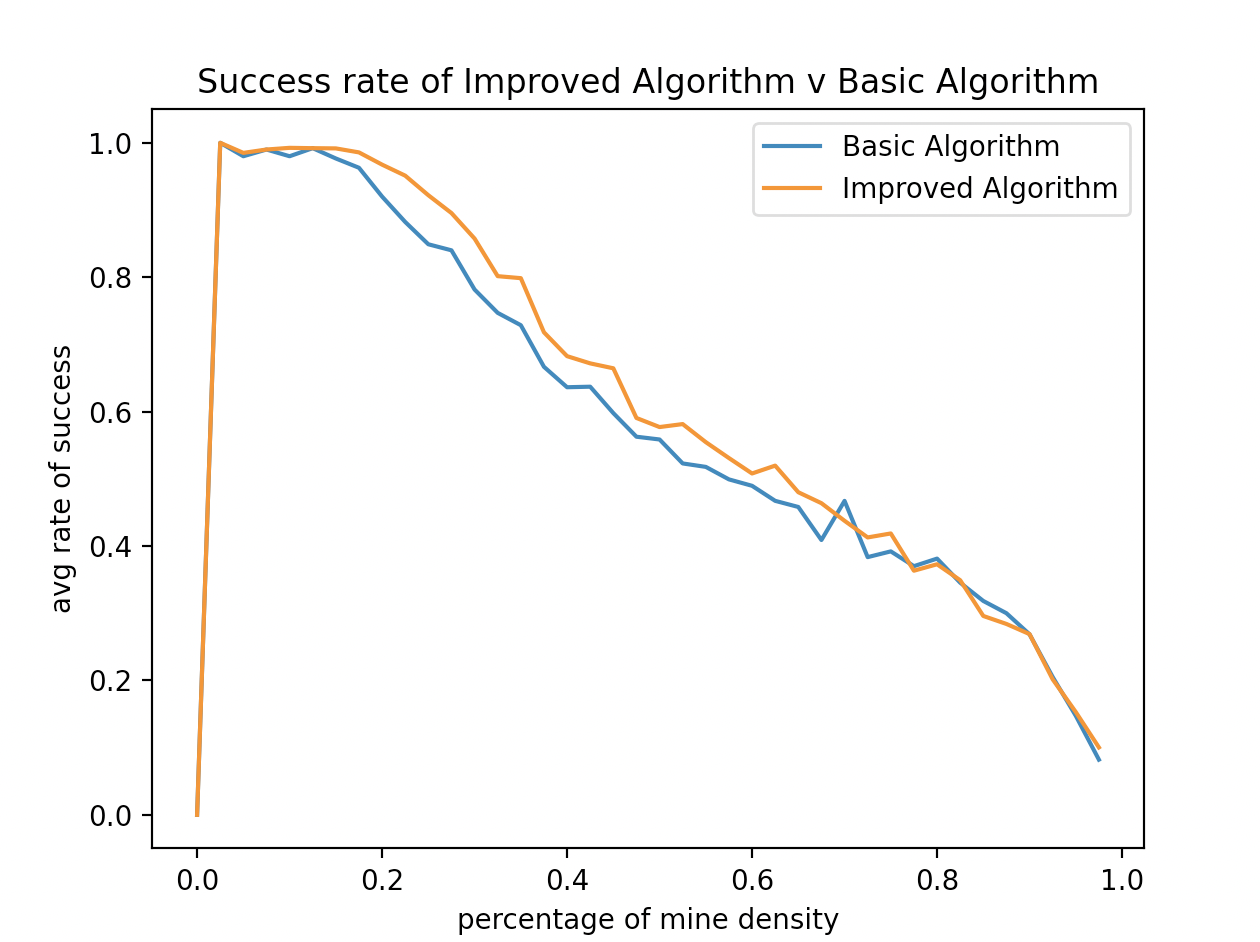
\includegraphics[width=0.7\textwidth]{images/performance_plot.png}}{No Figure Yet}
% 	\includegraphics[width=12cm]{dim100,50avg,step01}
	\caption{Plot of a function of mine density and the average final score (safely identified mines / total mines) for the simple baseline algorithm and our improved algorithm for comparison using a dimension of 20 and average of 10 random boards per given mine density}
	\end{figure}
	
	Our Strategy 3 algorithm SPOOFFs (Simulates Probability Of Our Future Fire) because TGIF(This Grid Is on Fire). It tries to account for unknown future by trying to predict the path of the fire. We do this in 2 ways. 
    \\\\
	1. We employ a deterministic approach where we assume the fire will spread 100\% of the time to all nodes it could possibly spread to for each time step. Based on this we generate a 3-D maze which has a maze for each time step. The size of the 3-D maze is dependent on the distance from the current position to the fire which is calculated using Manhattan distance. Based on the number of time steps we traverse through the 3-D maze and try to get as far as we can with a deterministic approach. 
	\\
	If this deterministic approach is unable to reach the goal, we use 2. 
	\\\\
	2. We employ a probabilistic approach where we assume where the fire will spread by generating an average of 10 possible mazes for each time step with the actual value of q. The average maze holds a probability for each cell catching on fire. Using each resulting average maze we generate a 3-D maze that holds an average maze for each time step, the number of time steps depending upon the distance of the current position on the path from the fire. From the last position of the path we traverse through the maze, choosing the cell that has the least probability of catching on fire at each time step.
	\\ 
	Once we have traversed the length of the time steps calculated using the distance from the fire, if we have not reached the goal we revert to the deterministic approach once again.
	\\\\
	Our strategy 3 is done using $A*$. $A*$ typically uses a heuristic value that is derived from calculating the euclidean distance of the current position from the goal and adding that to the traversed distance. This value is appended to a priority queue, where values are then chosen and dequeued based on their priority (smaller distances have higher priority). We altered this algorithm for strategy 3 by instead including a priority value that consisted of a tuple of 2 values. Our first value in the tuple consisted of the probability of that cell catching on fire, as calculated in our 3-D maze, summed with the probability of fire on that path so far. The second value in the tuple was of the distance heuristic (euclidean) that is typically used in $A*$. This tuple sorts the queue in ascending based on the first value and sub-sorts in ascending order based on the second value. We employed the use of a tuple in our priority queue because we wanted to prioritize survivability over getting the shortest possible path. 
	\\\\
	To optimize our algorithm and to preserve compute power we performed a $DFS$ algorithm on our initial maze before the fire has spread (time step = 0) to ensure that finish is reachable from start initially. Otherwise, it returns the maze because there is no possible path to finish.
	
\end{solution}

\smallskip

\textbf{Efficiency: }
What are some of the space or time constraints you run into in implementing this program? 
Are these problem specific constraints, or implementation specific constraints? 
In the case of implementation constraints, what could you improve on?


\smallskip

\begin{solution} \hfill
    \begin{figure}[h]
	\centering
	\IfFileExists{images/p6.png}{\includegraphics[width=1.1\textwidth]{images/p6.png}}{No Figure Yet}
% 	\includegraphics[width=12cm]{dim100,50avg,step01}
	\caption{} 
	\end{figure} 
	\begin{center}
	Strategy 1, Using a dimension of 100, average of 50, p=0.3, q with step of 0.1.
	
	Strategy 2, Using a dimension of 100, average of 50, p=0.3, q with step of 0.1.
	
	Strategy 3, Using a dimension of 10, average of 50, p=0.3, q with step of 0.1. 
    \end{center}
    
    Strategies 1, 2, and 3 perform the same from p = 0 to p = 0.2. Strategy 3 spikes up around p = 0.3. Strategy 1 has a higher value of success compared to Strategy 2 for p = 0.4. Strategy 3 has the highest success value at p = 0.6 and p = 0.9 compared to Strategies 1 and 2. This is because Strategy 3 should perform better than Strategies 1 and 2 with higher p values.
\end{solution}
\smallskip

\textbf{Global Information: }
	Suppose you were told in advance how many mines are on the board. Include this in your knowledge base. How did you model this? Regenerate the plot of mine density vs average final score with this extra information, and analyze the results.


\smallskip

\begin{solution} \hfill \\
	If we had unlimited computational resources we wouldn't need to rely on a deterministic approach to get a path. The purpose of our deterministic approach was to find a path from start to finish in less time because if there exists a path when q=1, that path exists for all other values of q. Using the deterministic approach in our algorithm reduces our computational power because using this approach does not require calculating an average of mazes. Therefore, we would completely rely on the probabilistic approach in order to find the path from start to finish. The probabilistic approach is a more accurate representation of the maze because it uses the real value of q instead of q=1 in order to sample what the fire looks like in future time steps. \\ \\
	Another approach we could take if we had unlimited computational resources is to calculate the state of the fire as far into the future as possible (i.e. until the goal can be reached). In our current algorithm, we calculate the number of time steps to look ahead in the future by how far we are from the fire currently. This caps how far we look into the future but if we had unlimited computational resources we would not need to place a limit on the number of steps to look ahead. \\ \\
    Lastly, we would want to increase the number of samples we use to average each probability maze for each time step. Currently, we are only sampling 10 mazes for each time step. By gathering more samples, we will have a more accurate picture of what the fire could look like at that time step. \\
\end{solution}

\smallskip

\textbf{Better Decisions: }
	In both the basic and improved agent, when nothing more could be inferred, the agent selects a covered cell at random. Build a better selection mechanism. How can you justify it? Regenerate the plot of mine density vs average final score with improved cell selection, and analyze the results.



\smallskip

\begin{solution} \hfill \\
     If we can only take 10 seconds between moves we would want to reduce the compute time our algorithm is taking. 
     \\\\
     Assuming the fire advances one step every 10 seconds, we would compute a path using BFS for as many neighboring layers we could reach within 5 seconds. From the last set of neighbors, we would compute the Manhattan distance from the goal and choose the path whose final layer leaves it closest to the goal. 
     \\\\
	 We would repeat this code until we either reach the goal, cannot move further due to a blockage, or the goal is on fire. 
	 We are assigning 5 seconds to get as far as we can with our path because we anticipate that calculating the Manhattan distance and path of each neighbor will have a time complexity of less than or equal to 5 seconds. 
	 
	 
% 	 If we can only take 10 seconds between moves we would want to reduce the compute time our algorithm is taking. A possible approach to this would be utilizing local search algorithms. The purpose of this would be because while finding the shortest path within these constraints might be impossible, finding a solution that can work, albeit not optimally, is preferable. 
\end{solution}

\textbf{Work Distribution}
\\
The work is our own and not copied or taken from any other students. 
\\\\
To work on this project we would meet up over video calls daily and discuss problems and our solutions. One person would then screen share and code while the others would contribute and also assist in coding using the request remote control feature in zoom. We would alternate in screen sharing and upload to git for version control. 
\\\\
The report was done similarly. We each took on a plot and a question to complete on our own. We then met to complete the rest as a group over video call. 
\\
$Asma$ $Makhdoom:$ Problem 2
\\
$Aamna$ $Farooq:$ Problem 3
\\
$Nada$ $Elshamaa:$ Problem 4 and Problem 6
\\
\smallskip

\end{document}